\documentclass[a4paper]{article}

\usepackage[pages=all, color=black, position={current page.south}, placement=bottom, scale=1, opacity=1, vshift=5mm]{background}
\SetBgContents{
    \tt This work is shared under a \href{https://creativecommons.org/licenses/by-sa/4.0/}{CC BY-SA 4.0 license} unless otherwise noted
}      % copyright

\usepackage[margin=1in]{geometry} % full-width

% AMS Packages
\usepackage{amsmath}
\usepackage{amsthm}
\usepackage{amssymb}

% Unicode
\usepackage[utf8]{inputenc}
\usepackage{hyperref}
\hypersetup{
    unicode,
%    colorlinks,
%    breaklinks,
%    urlcolor=cyan, 
%    linkcolor=blue, 
    pdfauthor={Héctor Climente-González, Chloé-Agathe Azencott},
    pdftitle={A simple article template},
    pdfsubject={A simple article template},
    pdfkeywords={article, template, simple},
    pdfproducer={LaTeX},
    pdfcreator={pdflatex}
}

% Vietnamese
%\usepackage{vntex}

% Natbib
\usepackage[sort&compress,numbers,square]{natbib}
\bibliographystyle{plainnat}

\usepackage{graphicx, color}
\graphicspath{{fig/}}

%\usepackage[linesnumbered,ruled,vlined,commentsnumbered]{algorithm2e} % use algorithm2e for typesetting algorithms
\usepackage{algorithm, algpseudocode} % use algorithm and algorithmicx for typesetting algorithms
\usepackage{mathrsfs} % for \mathscr command

% Author info
\title{martini: an R package for genome-wide association studies using SNP networks}
\author{Héctor Climente-González$^{1*}$ \and Chloé-Agathe Azencott$^{1,2}$}

\date{
\raggedright{
\small{
    $^1$RIKEN AIP \\
    $^2$MINES ParisTech, PSL Research University, CBIO-Centre for Computational Biology, F-75006 Paris, France;\\
    $^3$ Institut Curie, PSL Research University, F-75005 Paris, France;\\
    $^4$ INSERM, U900, F-75005 Paris, France;\\
%    \today
}
$^*$Corresponding author: \href{hector.climente@riken.jp}{hector.climente@riken.jp}\\
}
}

\begin{document}
    \maketitle
    
    \begin{abstract}
        
        We introduce \emph{martini}, an R package to build and analyze SNP co-function networks. Those are networks that model the genome by connecting SNPs if there is evidence they jointly contribute to the same biological function. \emph{Martini} builds such networks using three sources of information: sequential location, gene annotation, and gene-gene interactions. Such SNP networks involve hundreds of thousands of nodes, and millions of edges. To explore them, \emph{martini} implements two algorithms designed to scale to them: SConES and SigMod. Both algorithms seek a small subset of SNPs with high association scores with the phenotype of interest, and densely interconnected with each other in the network. Both algorithms require finding the optimal parameters. For that purpose, we implement a cross-validated grid search and three ways of scoring the solutions (stability, log-likelihood penalized metrics, and network properties). Lastly, \emph{martini} includes tools to visualize the network and association properties of the selected SNPs. \emph{Martini} is available on GitHub (\href{https://github.com/hclimente/martini}{hclimente/martini}) and Bioconductor (\href{https://www.bioconductor.org/packages/release/bioc/html/martini.html}{martini}).
        
        \noindent\textbf{Keywords:} gwas, networks, R 
    \end{abstract}

    \tableofcontents
    
    \section{Introduction}
    
    Networks are a widely used to formalize known relationships between biomolecules. Applied to human genetics, modeling the human genome through functional relationships between SNPs is useful to identify new causal SNPs and generate hypotheses \cite{climente-gonzalezBiologicalNetworksGWAS2020}. In this article, we introduce \emph{martini}, an R package that provides tools to build and analyze SNP networks.
    
    \section{Main functionalities}
    
    \begin{figure}[ht]
    \centering
    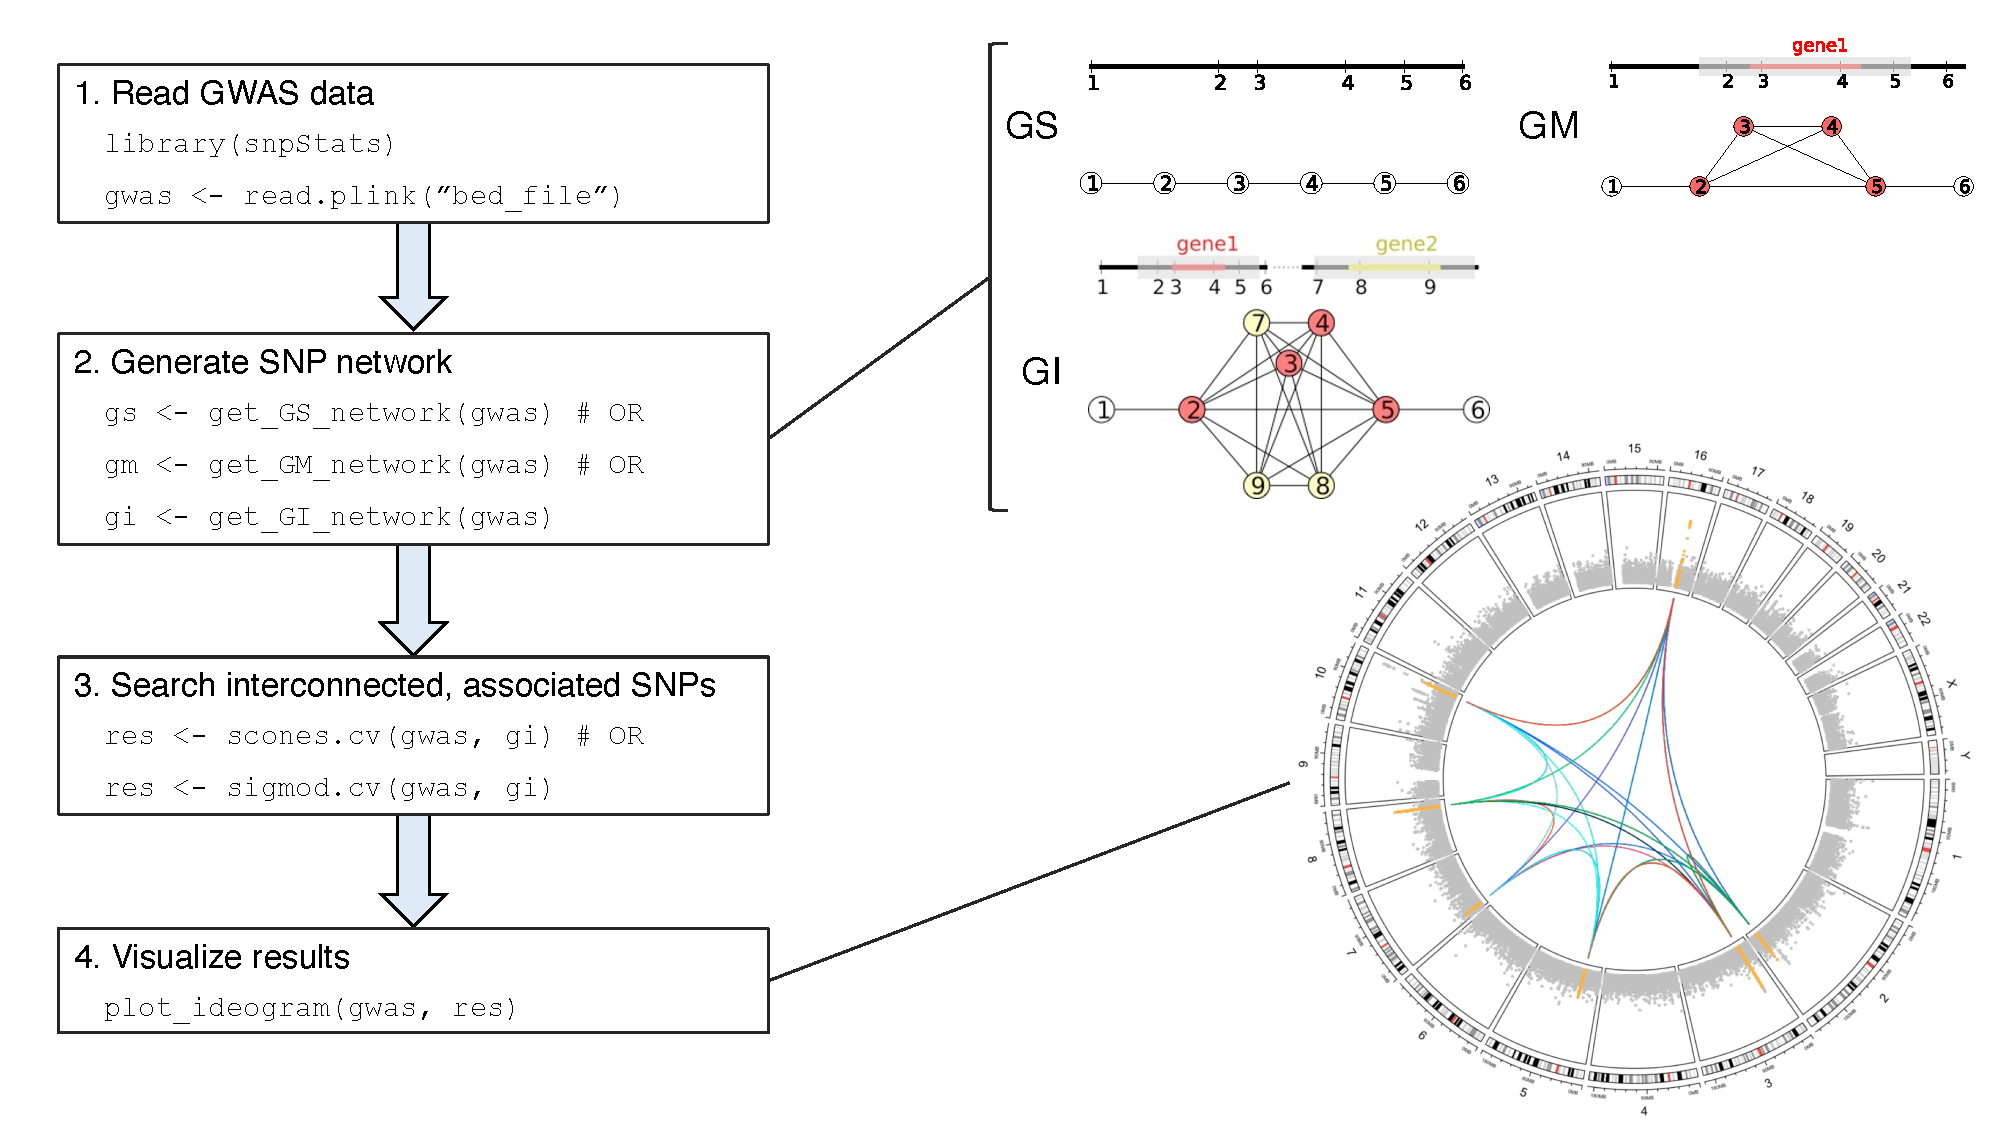
\includegraphics[width=\linewidth]{figure_1.pdf}
    \caption{Overview of a the 4 main steps of a \emph{martini} analysis. Adapted from Azencott \emph{et al.} \cite{azencottEfficientNetworkguidedMultilocus2013}.}
    \label{fig:overview}
    \end{figure}
    
    In the following sections, we present the different functionalities of \emph{martini} (see Fig \ref{fig:overview} for an overview).
    
    \subsection{Building SNP networks}
    
    In SNP networks, nodes are SNPs, which are connected by edges when there is some evidence of shared biological function between them. In principle, they can be built from any source of evidence of such shared functionality. \emph{Martini} includes functions to generate the three SNP networks described in Azencott \emph{et al.} \cite{azencottEfficientNetworkguidedMultilocus2013}, so-called GS, GM and GI (Fig \ref{fig:overview}):
    
    \begin{itemize}
    \item \texttt{get\_GS\_network()} provides the GS network, in which SNPs are connected if they are adjacent in the chromosome. 
    \item \texttt{get\_GM\_network()} produces the GM network, which includes the GS network and, in addition, all SNPs that are physically mapped to the same gene are interconnected.
    \item \texttt{get\_GI\_network()} generates the GI network, which includes the GM network and, on top of it, interconnects all the SNPs mapped to two genes that establish a protein-protein interaction.
    \end{itemize}
    
    The two latter functions require the user to provide mappings of SNPs to genes, and lists of gene-gene interactions. Conveniently, \emph{martini} provides easy ways of obtaining them via \texttt{snp2ensembl()} (map SNPs to the overlapping Ensembl genes) and \texttt{get\_gxg()} (recover gene-gene interactions from the BioGRID \cite{oughtredBioGRIDDatabaseComprehensive2020} and STRING \cite{szklarczykSTRINGV11Protein2019}). Importantly, different mappings can be used to generate SNP networks beyond those considered in Azencott \emph{et al.} \cite{azencottEfficientNetworkguidedMultilocus2013}. For instance, by providing a list of eQTLs, together with their target genes, \texttt{get\_GM\_network()} can generate networks based on gene expression regulation. Similarly, \texttt{get\_GI\_network()} can generate networks based on any type of gene-gene interaction beyond protein interactions.
    
    \subsection{Finding biomarkers using SConES and SigMod}

    \emph{Martini} implements two algorithms to search for connected subsets of SNPs associated to the phenotype: SConES \cite{azencottEfficientNetworkguidedMultilocus2013} and SigMod \cite{liuSigModExactEfficient2017}. They share the following formulation:

    \begin{eqnarray}
        \label{eq:scones}
        \underset{u \in\{0,1\}^{n}}{\arg \max } = \boldsymbol{c}^{T} \boldsymbol{u} - \lambda \boldsymbol{u}^{T} \boldsymbol{L} \boldsymbol{u} - \eta\|\boldsymbol{u}\|_{0},
    \end{eqnarray}
    
    where $u$ is a selection vector, in which element $u_i$ is 1 when SNP$_i$ is selected, and 0 otherwise; $c$ is a measure of association between the SNP and the phenotype; $L$ is the Laplacian matrix of the SNP network; and $\lambda$ and $\eta$ are parameters controlling connectivity and sparsity, respectively. In the case of SConES, $c = z$, where $z$ is a statistical measure of association between a SNP and the phenotype. For SigMod, however, $c = z + \lambda d$, where $d$ is the number of neighbors of the SNP in the network. In simple terms, this difference implies that SConES penalizes selecting a SNP but not its networks neighbors, while SigMod favors selecting both a SNP and its neighbors. In other words, SigMod prefers densely connected subnetworks, while SConES favors subnetworks relatively isolated from the rest. 
    
    \subsubsection{Parameter selection}

    Both SigMod and SConES require the selection of two parameters: $\lambda$ and $\eta$. If both are known, \emph{martini}'s functions \texttt{scones()} and \texttt{sigmod()} provide the corresponding subset of SNPs. Yet, in most cases, the optimal parameters of $\lambda$ and $\eta$ are unknown. For such cases, we provide the functions \texttt{scones.cv()} and \texttt{sigmod.cv()}. These functions explore a grid of parameters in a 10-fold cross-validated setting. For each combination of parameters an score is computed, using the average across the folds of a user-specified scoring function. Then, the best scoring set of parameters are used in a run on the whole dataset.
    
    \emph{Martini} includes three groups of scoring functions: stability, penalized log-likelihood, and network properties. \emph{Stability} selects the parameters that most consistently select the same SNPs across folds. \emph{Penalized log-likelihood} measures are computed on a linear model trained to predict the phenotype using exclusively the selected SNPs. They favor sets of SNPs that lead to good linear predictors, but penalize high complexities. Specifically, \emph{martini} has three such information criteria available: Bayesian, Akaike, and corrected Akaike (see Appendix \ref{app:llp_scores} for details). Lastly, \emph{network properties} include two measures that quantify the density of edges in the solution: the global, and the local clustering coefficients. 
    
    % TODO discuss hard threshold on number of selected SNPs
    
    Crucially, our implementation of SigMod is different from the one in the original paper \cite{liuSigModExactEfficient2017}, specifically the parameter selection.
    
    \subsubsection{Association tests}

    \emph{Martini} can perform two tests of statistical association between SNPs and the phenotype: 1 d.f. $\chi^2$ and generalized linear models (GLM). Using the former, the $\chi^2$ statistic is used as $z$ to compute $c$ in Eq \ref{eq:scones}; using the latter, regression coefficients are transformed into the corresponding $\chi^2$ statistic. Importantly, GLM allows to include additional user-specified covariates in the model, such as principal components to account for population structure.

    \subsection{Visualization}
    
    \emph{Martini} includes the function \texttt{plot\_ideogram()} to visualize the results on an ideogram composed of three layers (Fig \ref{fig:overview}). The first layer displays the cytobands. The second layer contains a circular Manhattan plot showing the the statistical association of each SNP. SNPs not selected by \texttt{scones.cv}/\texttt{sigmod.cv} are colored in gray, and selected SNPs in red. Lastly, the third layer displays the edges in the SNP network between SNPs from different chromosomes.
    
    \section{Implementation and availability}
    
    \emph{Martini} is implemented in R, and includes a fast C++ implementation of the min-cut/max-flow algorithm  \cite{boykovExperimentalComparisonMincut2004}. \emph{Martini} is available on GitHub (\href{https://github.com/hclimente/martini}{hclimente/martini}) and Bioconductor (\href{https://www.bioconductor.org/packages/release/bioc/html/martini.html}{martini}). The code is licensed as GPL-3. It includes vignettes to show the basic functionality.
    
    \section*{Funding and acknowledgments}

    This project was supported by funding from Agence Nationale de la Recherche (ANR-18-CE45-0021-01), the RIKEN Special Postdoctoral Researcher Program, and European Union’s Horizon 2020 research and innovation program (Marie Skłodowska-Curie [666003]). 

    \bibliography{bibliography}
    
    \newpage
    \appendix

    \section{Log-likelihood penalized scores}
    \label{app:llp_scores}
    
    Measures based on the accuracy of a linear classifier trained on the selected SNPs had been tested before, but exhibited proneness to overfitting. Hence we turned to penalized log-likelihood measures, developed in the field of information theory. These scoring functions had the potential to overcome the overfitting of a linear classifier by adding a regularization term to improve generalization. They take the form
    
    $$L(X,y,\hat{\theta})-c(\hat{\theta}),$$
    
    where $L(X,y,\hat{\theta})$ is the log-likelihood of the model, which depends on the feature matrix $X$, the outcome vector $y$, and the parameters $\hat{\theta}$; and $c(\hat{\theta})$ is a measurement of the model's complexity. Particularly, we explored three measures: Akaike information criterion (AIC), Bayesian information criterion (BIC), and corrected Akaike information criterion (AICc). All three take the form
    
    $$L(X,y,\hat{\theta})-\lambda p_{in},$$
    
    where $\lambda$ is a factor that controls the penalty for complexity; and $p_{in}$ is the number of features included in the model. Specifically they are defined as:
    
    $$ AIC=2L(X,y,\hat{\theta})-2p_{in} ,$$

    $$ BIC = -2L(X,y,\hat{\theta})-\ln(n)(p_{in}+ 2) ,$$

    and

    $$ AIC_c=AIC+\frac{2p_{in}(p_{in}+1)}{n-p_{in}-1}=-2L(X,y,\hat{\theta})+2\left(\dfrac{n}{n-p_{in}-1}\right)p_{in} .$$

    AICc is a modification of AIC that penalizes complex models (many features included) in high dimensional settings, that is, where the number of features is much larger than the number of samples, as in GWAS.
    
\end{document}